\chapter{$\tau$ tagging and calibration}

\section{Introduction}

%%%%%
% Need for a dedicated tau calibration
% ECAL/HCAL not perfect
% MET
% Calorimeter response
% collimated jet
% lots of ECAL
% Narrow jet - 0.4 cone instead of 0.5
% other properties i.e. lifetime - but i dont use it, so out in or not?
% tau decays - i.e. 1,3,5 prong
%%%%%

The $\tau$ lepton will be a useful signature of many physics processes at CMS. The $\tau$ decays via the weak mechanism with a characteristic decay time of $\tau$ = $290\times 10^{-15}$s ($c\tau$ = 87.11\micron)~\cite{pdg2006}. The $\tau$ primarily decays hadronically with a branching ratio of 65\%, forming a $\tau$ jet. When the jet has large transverse momentum, $\PT \gg M_{\tau}$ (1.78~\GeVcc), the constituent hadrons' momentum transverse to the jet axis is small resulting in a highly collimated, narrow jet. 77\% of hadronic decays consist of a single charged hadron and a number of neutral pions (one prong decays). The majority of the remainder of the hadronic decays involve 3 charged particles(three prong decays). Decays with 5 charged particles also occur but are much rarer.

The standard CMS reconstruction cone size ($\mathrm R = 0.5$) was too large for $\tau$ jets, introducing detector noise. Consequently this was optimised during this study. Figure~\ref{fig:tau_scale_cone_size} shows the energy containment and resolution, $\sigma(E)/<E>$, for $\tau$ jets as a function of reconstruction cone size for various \ETMC ranges. These plots show that a cone size of 0.4 was appropriate for $\tau$ jets, with a 98\% energy containment and good resolution.

\begin{figure}[tb]
  \centering
  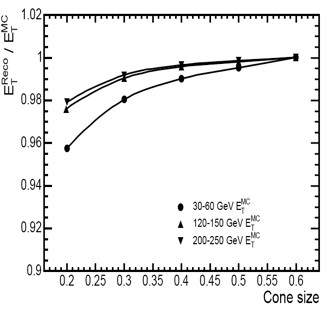
\includegraphics[width=0.49\textwidth]{tau/tautag_cont_vs_cone}
  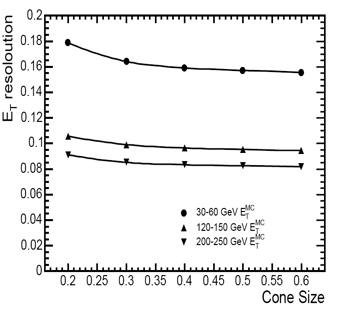
\includegraphics[width=0.49\textwidth]{tau/tautag_res_vs_cone}
  \caption{The $\tau$ jet energy scale, normalised to that obtained with a 0.6 cone, (left plot) and resolution, $\sigma/<E>$, (right plot) as a function of reconstruction cone size.~\cite{CMS_TDR_PHYS_vol1, citeulike:800614}
  \label{fig:tau_scale_cone_size}}
\end{figure}

\section{$\tau$ tagging}

%%%%%
% Tracker isolation - same Z vertex - IP cut to remove fake tracks
% ECAL isolation
% HLT CaloPxl
% impact paramater and tau mass and flight-path
%%%%%

A number of $\tau$ tagging methods have been developed for CMS \cite{CMS_TDR_PHYS_vol1, citeulike:800614}. Some of the most common techniques are presented below.

\subsection{Tracker isolation~\label{sec:tracker_isolation}}
\begin{figure}[!hHtb]
  \centering
  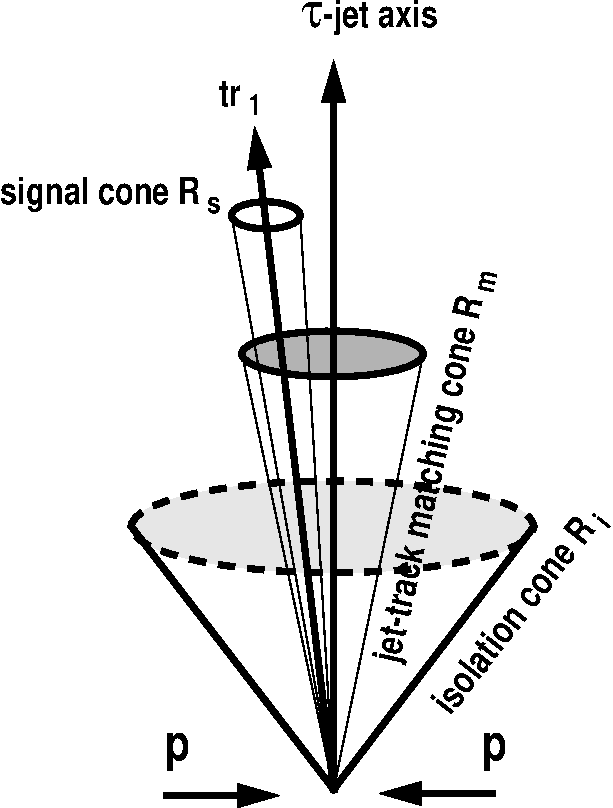
\includegraphics[width=0.45\textwidth]{tau/tautag_sketch_tauisol}
  \caption{$\tau$ identification method using the tracker.~\cite{CMS_TDR_PHYS_vol1, citeulike:800614}
  \label{fig:tracker_isol_sketch}}
\end{figure}

The tracker isolation method sought a narrow isolated $\tau$ jet. The principle is shown in Figure~\ref{fig:tracker_isol_sketch}. Tracks with \PT greater than a defined value, $\mathrm{p_{T}^{m}}$, with respect to the beam were sought within a matching cone of radius $\mathrm{R_{m}}$ about the calorimeter jet axis. The highest \PT track with unsigned transverse impact parameter $\mathrm{IP_{T} < 300}$\micron was defined to be the leading track ($\mathrm{tr_{1}}$). The $\mathrm{IP_{T}}$ cut removed fake tracks reconstructed from hits left by soft particles in QCD jets~\ref{fig:tau_ip}. Tracks within the cone $\mathrm{R_{S}}$ centred on $\mathrm{tr_{1}}$  with a z-impact parameter $\mathrm{z_{tr}}$ close to the z-impact parameter of the lead track $\mathrm{z_{tr}^{ltr}}$ ($\mathrm{|z_{tr} - z_{tr}^{ltr}| < \Delta z_{tr}}$) were assumed to come from the $\tau$ and termed ``signal tracks''. Other tracks within the cone $\mathrm{R_{i}}$ with $\mathrm{P_{T}}$ w.r.t the beam greater than $\mathrm{P_{T}^{i}}$ and satisfying $\mathrm{|z_{tr} - z_{tr}^{ltr}| < \Delta z_{tr}}$ were termed ``isolation tracks''. The isolation criteria required zero isolation tracks.

\begin{figure}[htb]
  \centering
  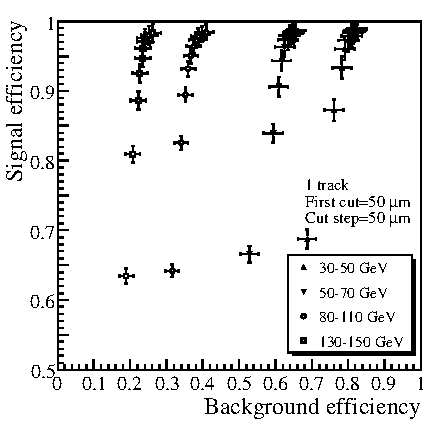
\includegraphics[width=0.49\textwidth]{tau/tautag_ip2d_1.pdf}
  \caption{$\tau$ tagging efficiencies for 1-prong $\tau$ jets and 4 \ETMC bins of 1-prong QCD multi jets. \ETMC obtained with Monte Carlo  particle jets excluding neutrinos. The upper cut on transverse impact parameter of the lead track is varied between $50-550~\micron$.~\cite{CMS_TDR_PHYS_vol1, citeulike:800614}
  \label{fig:tau_ip}}
\end{figure}

\begin{figure}[tb]
  \centering
  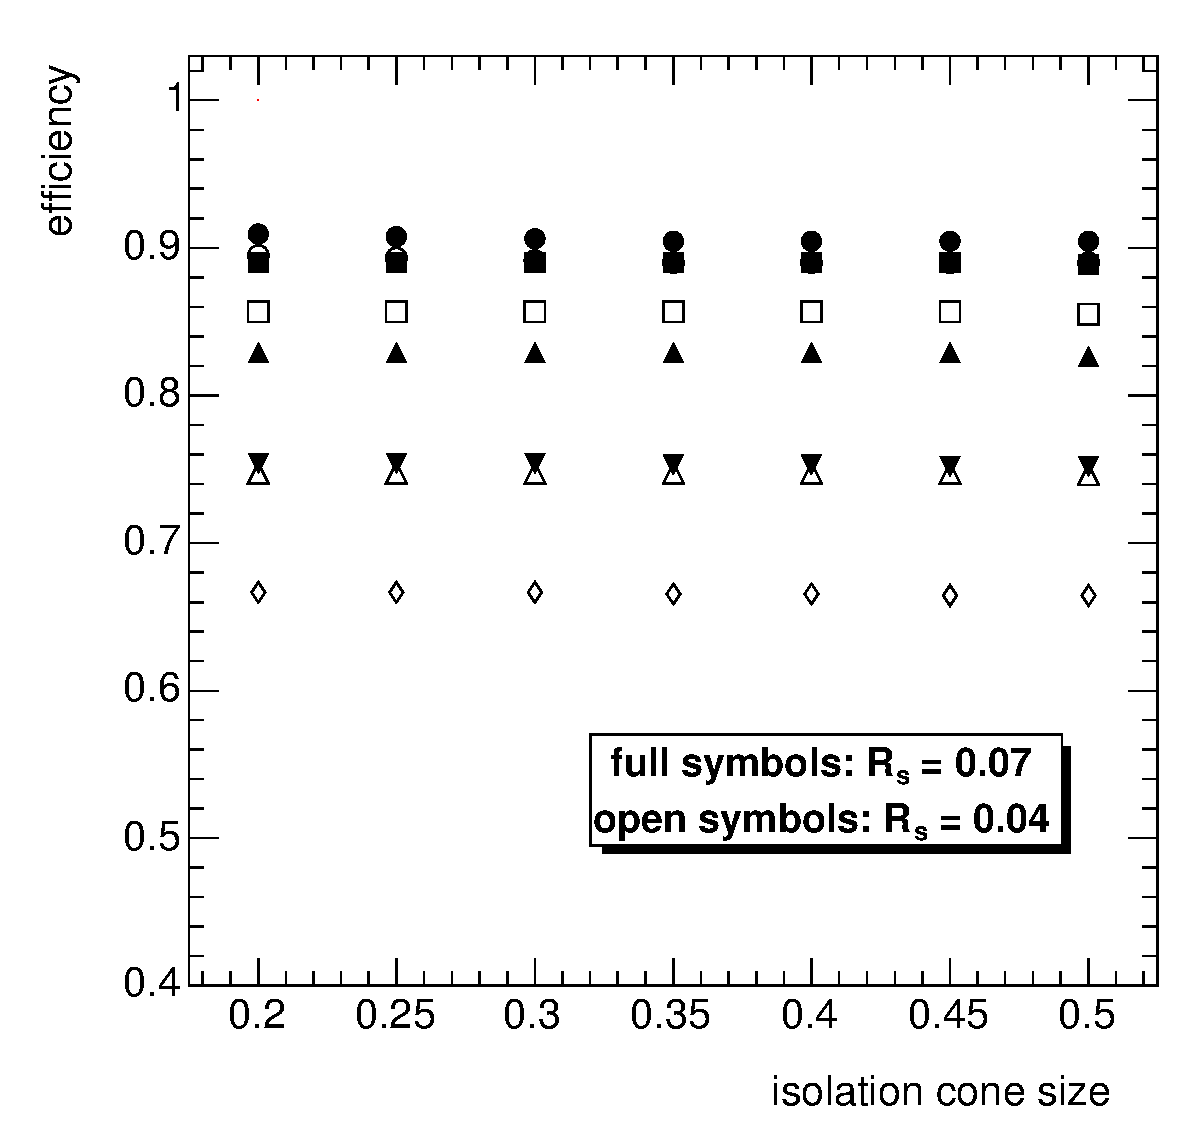
\includegraphics[width=0.45\textwidth]{tau/tautag_trkisol_tau}
  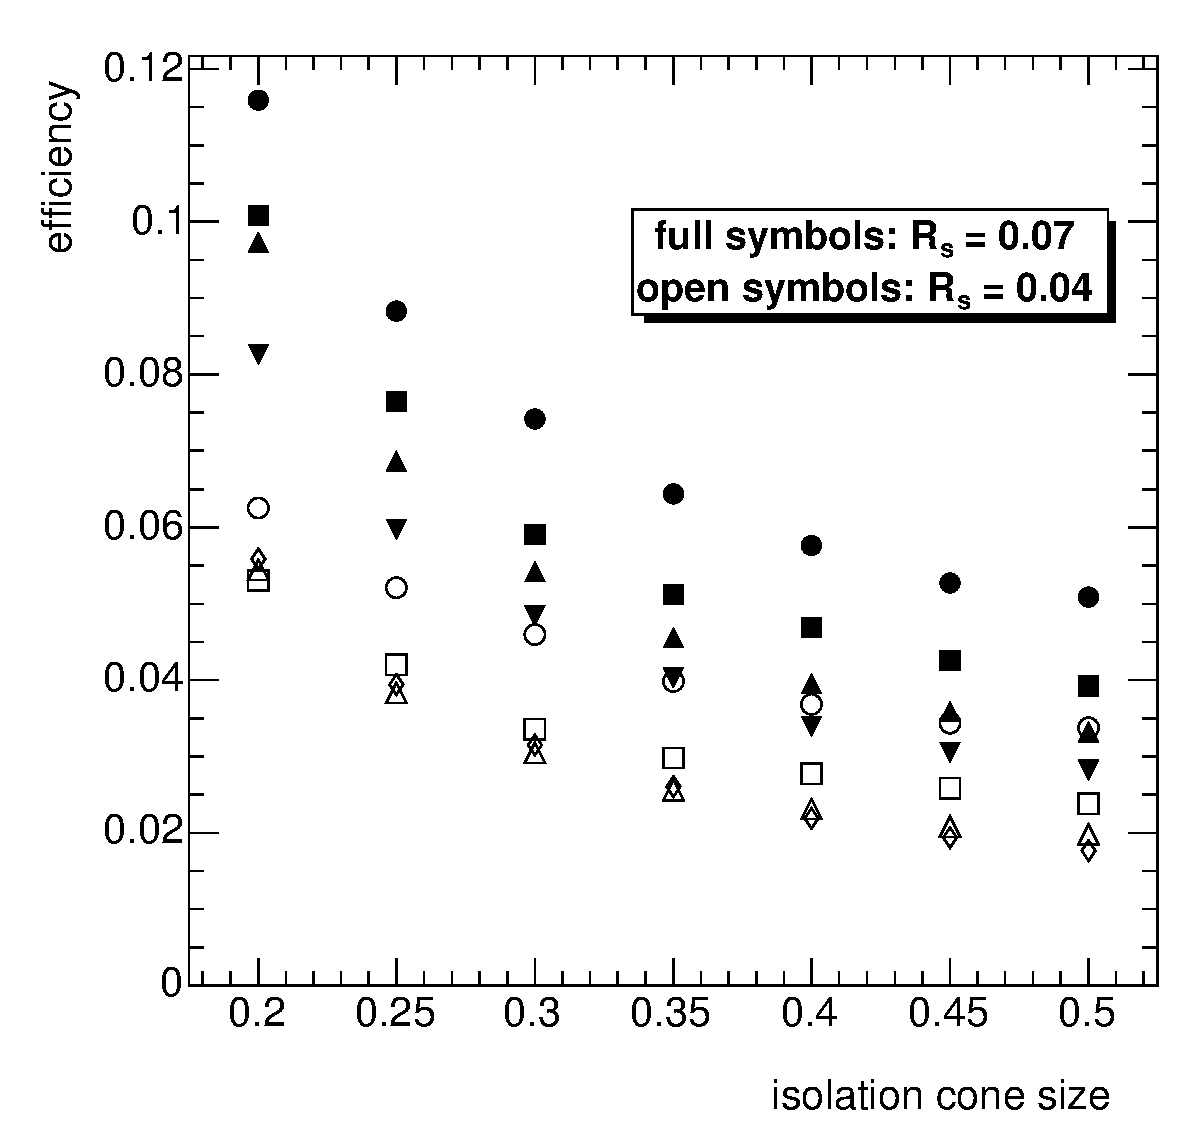
\includegraphics[width=0.45\textwidth]{tau/tautag_trkisol_qcd}
  \caption{The tracker isolation efficiency for $\tau$ jets (left plot) and
          QCD multi-jets (right plot) as a function of the isolation cone
          $\mathrm{R_{i}}$ for 2 values of the signal cone
          $\mathrm{R_{S}}$=0.07 (full symbols) and  $\mathrm{R_{S}}$=0.04
         (open symbols). In order of decreasing efficiency the symbols
          correspond to particle level jet \ETMC bins of 130--150, 80--110,
          50--70 and 30--50 GeV. The remaining tracker isolation parameters were:
          $\mathrm{R_{m}}$=0.1, $\mathrm{p_{T}^{i}}$=1\GeVc .
          $\mathrm{\Delta z_{tr}}$=2 mm and the leading track
          $\mathrm{p_{T}}>$ 6\GeVc.~\cite{CMS_TDR_PHYS_vol1, citeulike:800614}
  \label{fig:tautag_trkisol}}
\end{figure}

Figure~\ref{fig:tautag_trkisol} shows the tracker isolation efficiency for both $\tau$ and QCD jets. Jets were reconstructed using an iterative cone algorithm with a cone size of 0.4. Tracks were reconstructed with the combinatorial track finder algorithm (the standard CMS tracking algorithm~\cite{CMS_TRKTDR}) and were required to have at least 8 reconstructed hits, 2 in the pixel detector, and a $\chi^{2} < $ 10. Tracker isolation parameters used were: $\mathrm{R_{m}}$= 0.1, $\mathrm{p_{T}^{i}}$= 1\GeVc, $\mathrm{\Delta z_{tr}}$= 2 mm and the leading track $\mathrm{p_{T}}>$ 6\GeVc. It can be seen that the efficiency of genuine $\tau$ jets was independent of $\mathrm{R_{i}}$, for the studied range, whereas QCD multi-jet rejection increased with isolation cone size. 

The well-defined number of charged particles in a $\tau$ decay lead naturally to a requirement on the number of signal tracks of 1 or 3. The effect of this can be seen in Table~\ref{tab:tautag_nprongs}. From this it was concluded that the requirement on the number of signal tracks did not significantly improve QCD multi-jet rejection vs signal efficiency.

\begin{table}[tpb]
\begin{center}
\begin{tabular}{|l|c|c|c|c|}
\hline
QCD jets; \ETMC (GeV)
& 30--50 &  50--70 & 80--110 & 130--150  \\
\hline
1 track
& 63 \%  & 72 \%  & 69 \%  & 60 \%   \\
\hline
3 tracks
&  7 \%  &  9 \%  &  9 \%  & 13 \%   \\
\hline
1 or 3 tracks
& 70 \% &  81 \%  & 78 \%  & 73 \%      \\
\hline
\hline
$\tau$ jets; \ETMC (GeV)
& 30--50 &  50--70 & 80--110 & 130--150  \\
\hline
1 track
& 81 \% & 77 \%  & 71 \%  &  70 \%   \\
\hline
3 tracks
& 10 \% & 16 \%  & 16 \%  &  20 \%   \\
\hline
1 or 3 tracks
& 91 \% & 93 \%  & 87 \%  &  90 \%    \\
\hline
\end{tabular}

\caption{The efficiency of the track counting requirement for $\tau$ and
QCD jets in different bins of \ETMC.~\cite{CMS_TDR_PHYS_vol1, citeulike:800614}
\label{tab:tautag_nprongs}}
\end{center}
\end{table}

%To further suppress low \ET QCD jets a cut on the lead track \PT > 6 \GeVc could be used.

\subsection{Electromagnetic calorimeter isolation}
$\tau$ jets produce a narrow energy deposit in the electromagnetic calorimeter. The electromagnetic isolation $\mathrm{P_{isol}}$ parameter was found to provide the best hadronic jet rejection~\cite{CMS_TDR_PHYS_vol1, citeulike:800614}. Where $\mathrm{P_{isol}}$ was defined as

\begin{equation}
\mathrm{ P_{isol} = \sum_{\Delta R < 0.40}E_{T} - \sum_{\Delta R < 0.13}E_{T} }
\end{equation}

Jets with $\mathrm{P_{isol} < P_{isol}^{cut}}$ were considered $\tau$ candidates. Figure~\ref{fig:tautag_ecal_isol} shows how the efficiency for $\tau$ and QCD multi-jets jets
 varied with $\mathrm{P_{isol}^{cut}}$. Generally a value of 5 GeV was recommended for offline analysis.

\begin{figure}[tb]
  \centering
  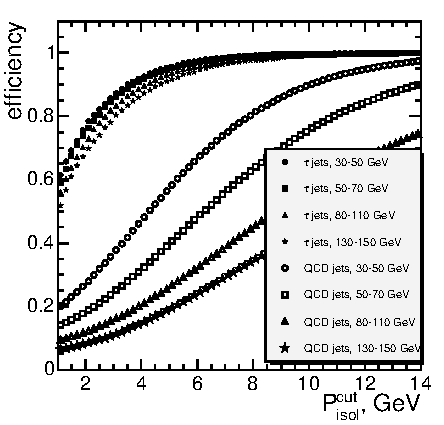
\includegraphics[width=0.55\textwidth]{tau/tautag_ecal_isol}
  \caption{Electromagnetic calorimeter isolation efficiencies for $\tau$ and QCD multi-jets as a function of $\mathrm{P_{isol}^{cut}}$.~\cite{CMS_TDR_PHYS_vol1, citeulike:800614}
  \label{fig:tautag_ecal_isol}}
\end{figure}

\subsection{Electron rejection \label{sec:e_rejection}}
An isolated electron (from a leptonic $\tau$ decay for instance) could pass both the $\tau$ jet tracker and electromagnetic isolation criteria. An offline cut on the most energetic HCAL tower in the jet was introduced to suppress these. Figure~\ref{fig:tau_e_reject} shows the hottest (maximal \ET) HCAL tower for 35 \GeV electrons and 2 \PT ranges of $\tau$s. The high electron \ET tail was due to electrons passing through $\eta-\phi$ ECAL gaps and the instrumentation gap between the barrel and endcap. Table~\ref{tab:tautag_etau_reject} shows the efficiency of this cut for $\tau$ jets and electrons. 

\begin{figure}[tb]
  \centering
  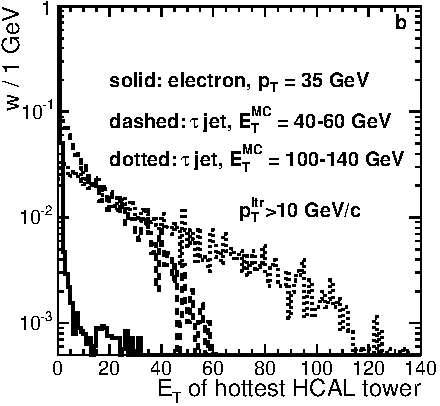
\includegraphics[width=0.45\textwidth]{tau/tautag_e_tau_reject}
  \caption{Transverse energy of maximal $E_{T}$ HCAL tower (\GeV). All histograms are normalised to unity.~\cite{CMS_TDR_PHYS_vol1, citeulike:800614}
  \label{fig:tau_e_reject}}
\end{figure}

$\mu$ lepton rejection was not investigated as energy deposited in the calorimeter was only of the order of a few \GeV, well below the jet \ET cuts used in most CMS analyses.
%%%%%%
% Move to detector chapter
%\subsection{Level-1 trigger}
%The $\tau$ trigger uses the same sliding 3 $\times 3$ window of $4 \times 4$ trigger towers as the jet trigger. Figure shows the acceptable $\tau$ energy deposit shapes. This algorithm is only applied within the region $|\eta| < 1.95$ and the jet energy is taken as the sum of the central tower.
%%%%%

\subsection{High Level Trigger\label{sec:CaloPxl}}
The High Level Trigger utilised both ECAL and tracker isolation. The HLT $\tau$ trigger was optimised for the MSSM heavy Higgs boson decaying to 2 hadronic $\tau$ jets.

\begin{table}[tb]
  \begin{tabular}{|l|c|c|c|c|c|}
   \hline
& & \multicolumn{2}{|c|}{$\tau$ jet $E_{\rm T}$ 40--60 GeV} &
    \multicolumn{2}{|c|}{$\tau$ jet $E_{\rm T}$ 100--140 GeV} \\
    \cline{3-6}
    \raisebox{1.5ex}[0cm][0cm]{cut} &
    \raisebox{1.5ex}[0cm][0cm]{electron} &
        $p_{\rm T}^{\rm ltr}>$ 10 GeV &
        $p_{\rm T}^{\rm ltr}>$ 25 GeV &
        $p_{\rm T}^{\rm ltr}>$ 10 GeV &
        $p_{\rm T}^{\rm ltr}>$ 25 GeV \\
   \hline
$>$1 GeV & 0.08 & 0.936 & 0.971 & 0.977 & 0.991 \\
   \hline
$>$2 GeV & 0.03 & 0.854 & 0.917 & 0.942 & 0.969 \\
   \hline
  \end{tabular}
  \caption{Efficiency of the transverse energy of the hottest
           HCAL tower (maximal \ET) cut for electrons \PT = 35 \GeVc and
           for different $\tau$ jet \PT ranges and lead track \PT ($\mathrm{p _{\rm T} ^{\rm ltr}}$).~\cite{CMS_TDR_PHYS_vol1, citeulike:800614}}
  \label{tab:tautag_etau_reject}
\end{table}

The recommended HLT algorithm, ``Calo+Pxl'',~\cite{CMS_TDR_PHYS_vol1, citeulike:800614} relied on ECAL isolation followed by tracker isolation using only the pixel layers. This algorithm took as seeds the 2 Level-1 $\tau$ primitives. If no second candidate was identified the most energetic Level-1 central jet candidate was considered.

\begin{figure}[tb]
\centering
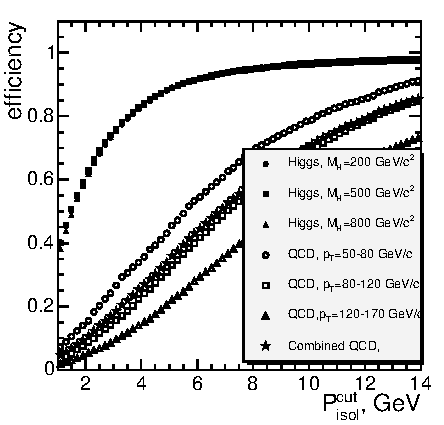
\includegraphics[width=0.55\textwidth]{tau/tautag_ecalisol_hlt}
\caption{The efficiency of the ECAL isolation at the High Level Trigger for 
         the signal and the QCD multi-jet background as a function of the cut 
         $\mathrm{P _{\rm isol}^{\rm cut}}$ on the ECAL isolation parameter.~\cite{CMS_TDR_PHYS_vol1, citeulike:800614} }
\label{fig:tautag_ecalisol_hlt}
\end{figure}

Figure~\ref{fig:tautag_ecalisol_hlt} shows the efficiency of the ECAL isolation criteria for $\tau$ jets and multi-jets. A reduction in the multi-jet rate of $\sim$ 3 was achieved with $\mathrm{P_{isol}^{cut}} = 5 \GeV$.

Jets that passed the calorimeter isolation were passed through tracker isolation with the pixel detector. Track candidates were formed from hit pairs in the first two pixel layers. Quality cuts were applied consistent with a track \PT of 1 \GeVc or above. Hits from the third pixel layer were combined with the track candidates to form pixel-tracks. A list of primary vertices was formed from the pixel-track z impact parameters. Vertices associated with fewer than three pixel-tracks were discarded. Each vertex was computed as the mean of the z impact parameters of the constituent tracks.

The tracker isolation was then run with the pixel-tracks. The lead track was required to have $\mathrm{p_{T}^{ltr}} > 3 \GeVc$ and to be within the cone $\mathrm{R_{m}} = 0.1$ around the jet axis. All further tracks were required to come from the same vertex as the lead track. Signal tracks were located within the cone $\mathrm{R_{S}}$=0.07 with no further tracks permitted within the isolation cone, $\mathrm{R_{i}}$.

\begin{figure}[!hHtb]
\begin{center}
\begin{tabular}{cc}
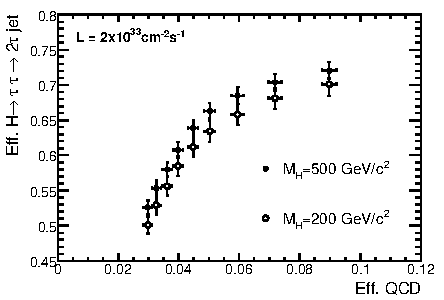
\includegraphics[width=0.49\textwidth]{tau/eff_hlt_pix_1stjet}
&
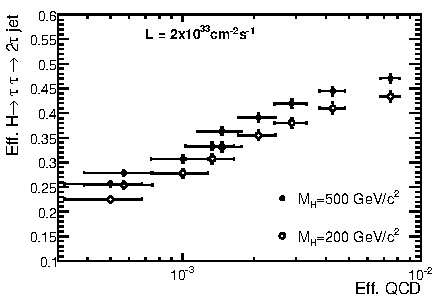
\includegraphics[width=0.49\textwidth]{tau/eff_hlt_pix_2jets}
\end{tabular}
    \caption{Efficiency of Calo+Pxl trigger applied to the 
             first jet (left) and to both jets (right) for signal 
             events versus efficiency for QCD multi-jet events. 
             Two Higgs boson masses of $\mathrm{M}_{\rm H}$=200 and 
             500 GeV/$c^{2}$ are shown. The isolation cone is varied from 0.2 to 
             0.6 in steps of 0.05; the signal cone is 0.07; the matching cone is 0.1; 
             and the $\PT$ of the leading tracks must exceed 
             3 GeV/$c$.~\cite{CMS_TDR_PHYS_vol1, citeulike:800614} 
}
\label{fig:pxl_eff}
\end{center}
\end{figure}

Figure~\ref{fig:pxl_eff} shows the Calo+Pxl single (left) and double (right) $\tau$ efficiencies for both H$\rightarrow \tau \tau$ and QCD multi-jets (50 $< \ETMC < 170 \GeV$) as a function of the isolation cone size. The A/H$\rightarrow \tau \tau$ analysis required a double trigger. It can be seen that a double trigger background rejection rate of $\sim 10^{-3}$ could be achieved with an $\mathrm{R_{i}}$ of 0.45--0.5, giving a signal efficiency of 0.29--0.32.

\section{$\tau$ jet energy scale}
Figures~\ref{fig:tau_scale} and~\ref{fig:jet_scale} show the $\tau$ and QCD multi-jet energy scales. The drop at $\eta~\simeq 1.4$ was due to the instrumentation gap between the calorimeter barrel and endcap sections. It can be seen that the $\tau$ energy scale was significantly higher than that of multi-jets. This was a consequence of the intrinsically higher electromagnetic response and the $\tau$ jets' low multiplicity. Both these resulted from $\tau$ jets being predominantly light quark jets containing neutral pions. Thus $\tau$ jets required a dedicated energy scale calibration.
%The highest response was from $\tau$ decays involving $\pi^{0}$s and a low number of $\pi^{\pm}$s. This was a consequence of the intrinsically higher electromagnetic response and the $\tau$ jets low multiplicity. Thus $\tau$ jets required a dedicated energy scale calibration.

\begin{figure}[tb]
  \centering
  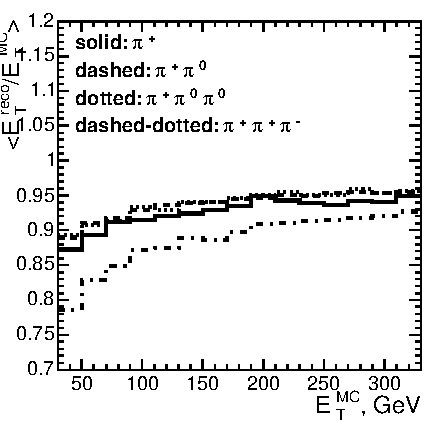
\includegraphics[width=0.49\textwidth]{tau/tautag_scalei_vs_pt}
  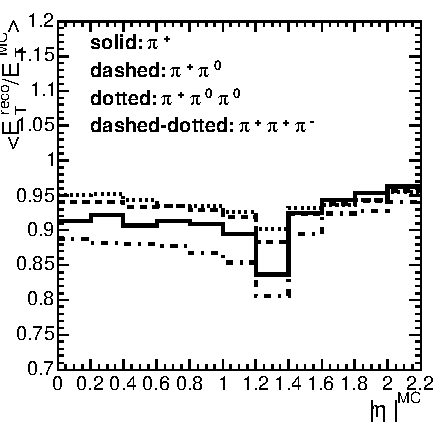
\includegraphics[width=0.49\textwidth]{tau/tautag_scalei_vs_eta}
  \caption{The Monte Carlo $\tau$ jet energy scale for different decay final states.~\cite{CMS_TDR_PHYS_vol1, citeulike:800614} 
  \label{fig:tau_scale}}
\end{figure}

\begin{figure}[!hHtb]
  \centering
  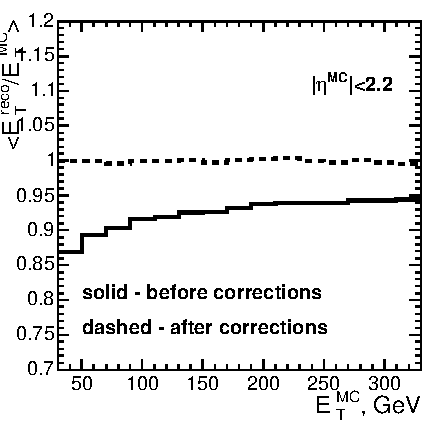
\includegraphics[width=0.49\textwidth]{tau/tautag_scale_vs_pt}
  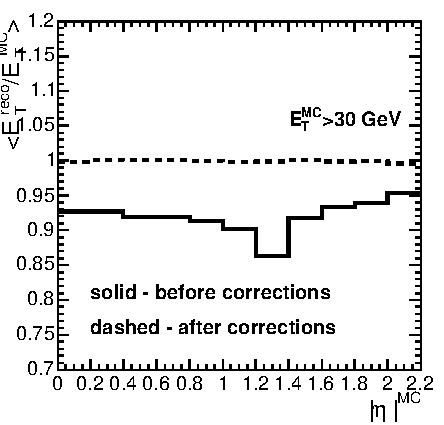
\includegraphics[width=0.49\textwidth]{tau/tautag_scale_vs_eta}
  \caption{Simulated $\tau$ jet \ET scale before and after Monte Carlo corrections for 1 and 3 pronged $\tau$ jets in the presence of low luminosity pileup.~\cite{CMS_TDR_PHYS_vol1, citeulike:800614}
  \label{fig:tau_scale_corr}}
\end{figure}

\subsection{Monte Carlo calibration~\label{sec:MC_tau_calib}}

%%%%%
% MC calibration method
% plots
% resoloution - compare standard qcd jets
%%%%%

A Monte Carlo $\tau$ jet energy calibration was developed in this study for use in Monte Carlo analyses. This correction was obtained from a parameterisation in $\eta$ and \ET of the ratio $\mathrm{E_{T}^{reco}/E_{T}^{MC}}$ for  Monte Carlo single prong, 3 prong and 1 + 3 pronged decays in the presence of pileup at an instantaneous luminosity of \lowlumi. Figure~\ref{fig:tau_scale_corr} shows the $\tau$ jet energy scale before and after calibration for 1 + 3 pronged $\tau$ jets.



\begin{figure}[tb]
  \centering
  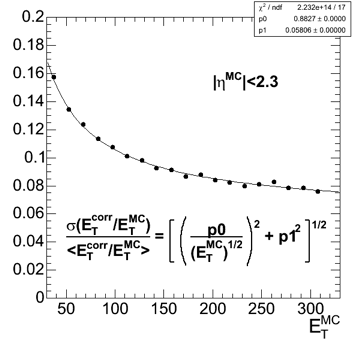
\includegraphics[width=0.65\textwidth]{tau/tau_resol}
  \caption{The calibrated $\tau$ jet \ET resolution in the presence of low luminosity pileup.~\cite{CMS_TDR_PHYS_vol1, citeulike:800614}
  \label{fig:tau_resol}}
\end{figure}

The energy resolution after the correction can be seen in Figure~\ref{fig:tau_resol} and parameterised as:

\begin{equation}
\mathrm{
\frac{\sigma\left(\frac{E_{T}^{corr}}{E_{T}^{MC}}\right)}{\langle\frac{E_{
	      T}^{corr}}{E_{T}^{MC}}\rangle}=\frac{0.883}{\sqrt{E_{T}^{MC}}} \oplus 0.058
}
\end{equation}

for $\tau$ jets with $E_{T}$ between 30 and 300 GeV and pseudorapidity less than 2.3. Figure~\ref{fig:Jet_perf} shows the comparative plot for QCD multi-jets.

\subsection{Proposal for calibration from data}

%%%%%
% gamma + jet calibration
% pass through tau id
% plots
%%%%%



Once CMS begins data taking a calibration from real data will be needed. One proposal for this involved taking Z $\rightarrow \tau \tau \rightarrow l + jet$ events and reconstructing the Z mass peak~\cite{CMS_TDR_PHYS_vol1}. The $\tau$ energy scale could be computed from the well known lepton energy scale and Z mass peak. Disadvantages of this approach included background contamination and the \MET resolution.

Another approach was proposed.~\cite{CMS_TDR_PHYS_vol1, citeulike:800614} and studied here, using $\gamma$ + jet events, which are already planned to be used to calibrate the QCD multi-jet energy scale. It has been proposed that those jets that pass the $\tau$ tagging criteria may have an energy scale similar to that of genuine $\tau$ jets. To evaluate the feasibility of this approach the QCD multi-jets sample was passed through the $\tau$ tagging criteria and the energy scale determined. Jets were reconstructed with cone size 0.4 and passed through both tracker and ECAL isolation. Isolation was performed with parameters $\mathrm{P_{isol}^{cut}}$=5 GeV, $\mathrm{R_{i}}$=0.4, $\mathrm{R_{S}}$=0.07, lead track \PT $>$ 10 \GeVc and with the requirement for 1 or 3 signal tracks. QCD multi-jets that passed all $\tau$ criteria were termed $\tau$ like. 

Figure~\ref{fig:tau_qcd_scale} shows the results. One can see that $\tau$ like jets had a much higher calorimeter response compared to untagged jets. However there was still a 5--10\% systematic offset. This is probably due to the same reasons that give $\tau$ jets there inherently high energy response. It is possible that this difference may be reduced when CMS adopts particle flow algorithms which could be used to select QCD jets that are even more similar to $\tau$ jets than the ones presently selected. If this approach does not provide similar responses an extra correction factor could be applied to the $\tau$-like jet energy scale. However this would introduce new errors and systematics and would therefore be undesirable.

\begin{figure}[tb]
  \centering
  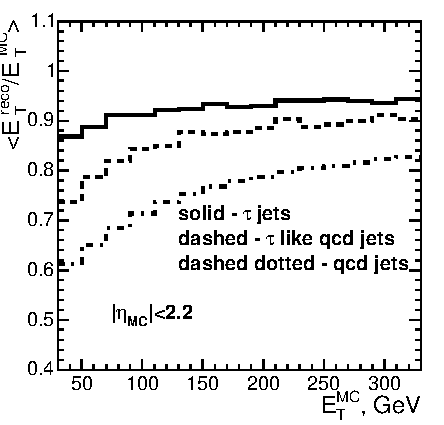
\includegraphics[width=0.45\textwidth]{tau/tautag_calibr_qcd_pt}
  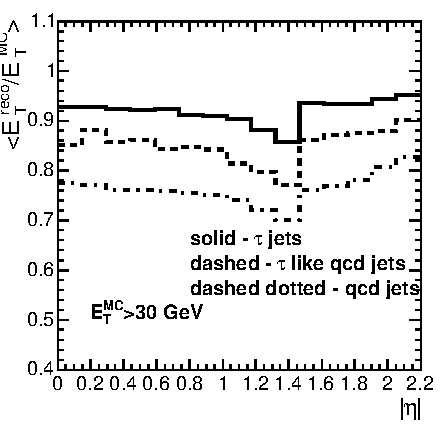
\includegraphics[width=0.45\textwidth]{tau/tautag_calibr_qcd_eta}
  \caption{The energy scale for $\tau$ jets, QCD multi-jets that pass the $\tau$ tagging criteria and jets which do not.~\cite{CMS_TDR_PHYS_vol1, citeulike:800614}
  \label{fig:tau_qcd_scale}}
\end{figure}

\begin{figure}[tb]
  \centering
  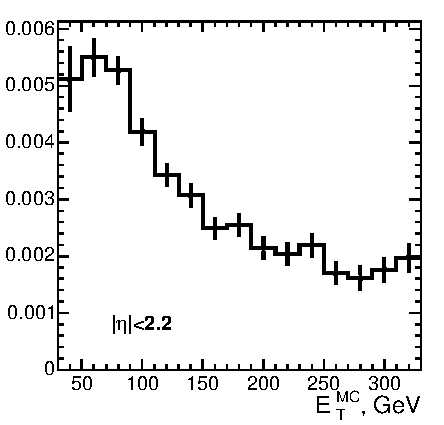
\includegraphics[width=0.45\textwidth]{tau/tautag_calibr_qcd_pt_eff}
  \caption{The efficiency for a QCD multi-jet to pass the $\tau$ tagging criteria.~\cite{CMS_TDR_PHYS_vol1, citeulike:800614}
  \label{fig:tau_qcd_eff}}
\end{figure}
The QCD multi-jet miss-tag efficiency as a function of \ET is shown in Figure~\ref{fig:tau_qcd_eff}.

\section{Conclusion}
The $\tau$ tagging and calibration performance are important for a number of physics channels at CMS. Multiple $\tau$ tagging methods have been developed for use in the High Level Trigger and offline analysis. A Monte Carlo jet energy calibration has been developed and a method proposed to obtain the calibration from data.
